\documentclass[conference]{IEEEtran}

% Packages
\usepackage{fontspec} % For XeLaTeX
\usepackage{xeCJK}    % For Chinese characters (if needed in future)
\usepackage{cite}
\usepackage{amsmath,amssymb}
\usepackage{algorithm}
\usepackage{algorithmic}
\usepackage{graphicx}
\usepackage{booktabs}
\usepackage{array}
\usepackage{multirow}
\usepackage{float}
\usepackage{url}
\usepackage{caption}
\usepackage{subcaption}

% Set main font and CJK font
\setmainfont{Times New Roman}
\setCJKmainfont{SimSun} % 宋體,請根據需求調整

% Title and author
\title{Global Search Strategy Based on Improved Hyper DE: A Comparative Analysis with Traditional Differential Evolution}

\author{
\IEEEauthorblockN{Tse-Lin Li}
\IEEEauthorblockA{
\textit{Department of Computer Science} \\
\textit{Fu Jen Catholic University} \\
New Taipei City, Taiwan \\
511172176@m365.fju.edu.tw}
}

\begin{document}

\maketitle

\begin{abstract}
With the widespread application of optimization problems in fields such as engineering design, machine learning, and operations research, metaheuristic algorithms have garnered significant attention due to their powerful global search capabilities. This paper focuses on the Hyper Differential Evolution (Hyper DE) algorithm, exploring its potential in diverse optimization problems and proposing a series of improvement strategies to enhance its search efficiency and solution quality. Specifically, by introducing diversity maintenance mechanisms, adaptive parameter control, and hybrid strategies, this study aims to bolster the performance of Hyper DE in handling high-dimensional and multimodal problems. The experimental section compares the performance of traditional Differential Evolution (DE) with the improved NewDE across multiple benchmark functions, analyzing their superiority in global search. Furthermore, this paper conducts a sensitivity analysis of the improvement strategies and discusses their potential value and future research directions in practical applications.
\end{abstract}

\begin{IEEEkeywords}
Metaheuristic Algorithms, Hyper Differential Evolution, Global Search, Differential Evolution, Adaptive Parameters, Hybrid Strategies
\end{IEEEkeywords}

\section{Introduction}

Optimization problems play a crucial role in modern science and engineering, impacting areas such as structural design, path planning, machine learning model training, resource allocation, and scheduling. The effectiveness of optimization methods directly influences system performance and efficiency. As problem scales and complexities increase, traditional optimization methods like gradient descent and linear programming often face challenges such as getting trapped in local optima and excessive computational resource consumption when dealing with non-convex, multimodal, and high-dimensional problems \cite{floudas1999review, pinter1996global, goldberg1989genetic, kennedy1995particle, storn1997differential, eiben1999parameter}. To address these challenges, metaheuristic algorithms have emerged as powerful tools due to their efficient global search capabilities and flexible adaptability \cite{burke2013hyper}.

Differential Evolution (DE) is a simple yet highly effective evolutionary computation method widely applied to various continuous optimization problems \cite{storn1997differential}. Hyper Differential Evolution (Hyper DE), an improved version of DE, incorporates ideas from Genetic Algorithms (GA) to dynamically adjust DE's hyperparameters, such as the mutation factor $F$, crossover rate $CR$, and population size $S$, thereby enhancing its adaptability and efficiency across diverse problem landscapes \cite{burke2013hyper, grobler2010alternative}. However, as optimization problems evolve and diversify, Hyper DE still encounters limitations, particularly in handling high-dimensional and multimodal problems where it is prone to local optima traps and exhibits sensitivity to parameter settings \cite{grobler2010alternative}.

Therefore, this paper aims to enhance Hyper DE by introducing diversity maintenance mechanisms, adaptive parameter control, and hybrid strategies to improve its global search capability and solution quality. The primary contributions of this paper are:

\begin{enumerate}
    \item Proposing diversity maintenance mechanisms to prevent premature convergence and preserve population diversity.
    \item Exploring adaptive parameter control strategies that dynamically adjust algorithm parameters based on search performance.
    \item Integrating hybrid strategies to leverage the strengths of different algorithms, thereby improving global search efficiency and effectiveness.
    \item Validating the superior performance of the improved NewDE over traditional DE in multimodal and high-dimensional problems through comprehensive experiments.
\end{enumerate}

\section{Literature Review}

\subsection{Overview of Metaheuristic Algorithms}

Metaheuristic algorithms are high-level heuristic methods designed to solve complex optimization problems, particularly those characterized by multimodality and high dimensionality \cite{burke2013hyper, grobler2010alternative}. Unlike problem-specific algorithms, metaheuristics do not rely on the problem's specific structure but instead emulate natural processes such as biological evolution and swarm intelligence to perform global searches. Common metaheuristic algorithms include Genetic Algorithms (GA), Particle Swarm Optimization (PSO), Simulated Annealing (SA), and Ant Colony Optimization (ACO) \cite{burke2013hyper, storn1997differential, eiben1999parameter, grobler2010alternative}.

\subsection{Particle Swarm Optimization (PSO) and Ant Colony Optimization (ACO)}

Particle Swarm Optimization (PSO) simulates the collective behavior of bird flocks or fish schools, where each particle represents a potential solution. Particles adjust their velocities and positions based on their personal best experiences ($pbest$) and the group's best experience ($gbest$) to achieve global search \cite{kennedy1995particle, storn1997differential}. PSO is praised for its simplicity and efficiency, especially in continuous optimization problems. However, PSO tends to converge prematurely to local optima when dealing with high-dimensional and multimodal problems \cite{eiben1999parameter}.

Ant Colony Optimization (ACO) models the foraging behavior of ants, utilizing pheromone trails to guide ants' path selection, thereby performing global searches \cite{kennedy1995particle, storn1997differential}. ACO excels in combinatorial optimization problems, such as the Traveling Salesman Problem (TSP), but suffers from higher computational complexity and sensitivity to pheromone parameter settings \cite{storn1997differential}.

\subsection{Differential Evolution (DE) and Hyper DE}

Differential Evolution (DE) is a population-based evolutionary algorithm that employs mutation, crossover, and selection operations to evolve candidate solutions toward the global optimum \cite{storn1997differential, eiben1999parameter}. DE is renowned for its simplicity, high efficiency, and minimal control variable requirements, making it widely applicable. Nevertheless, DE can struggle with high-dimensional and multimodal problems, often getting trapped in local optima and showing sensitivity to parameter configurations \cite{storn1997differential, eiben1999parameter}.

Hyper Differential Evolution (Hyper DE) is an enhanced version of DE that integrates Genetic Algorithm (GA) concepts to dynamically manage DE's hyperparameters, such as the mutation factor $F$, crossover rate $CR$, and population size $S$ \cite{burke2013hyper, grobler2010alternative}. The core idea of Hyper DE involves maintaining a population of DE instances, each with different hyperparameter settings, and evolving these hyperparameters through genetic operations like selection, crossover, and mutation to better suit the current search requirements \cite{burke2013hyper, grobler2010alternative}.

\subsection{Existing Improvements in Metaheuristic Algorithms}

Current improvements in metaheuristic algorithms primarily focus on the following aspects:

\begin{enumerate}
    \item \textbf{Adaptive Parameter Adjustment}: Dynamically tuning parameters such as mutation factors and crossover rates based on search performance to balance exploration and exploitation \cite{burke2013hyper, grobler2010alternative}.
    \item \textbf{Diversity Maintenance Mechanisms}: Introducing diversity indicators to monitor population diversity and implementing diversity-enhancing operations when diversity falls below a threshold to prevent premature convergence \cite{burke2013hyper, grobler2010alternative}.
    \item \textbf{Hybrid Strategies}: Combining different optimization methods (e.g., GA and SA) to harness their respective strengths, thereby improving global search capabilities, accelerating convergence, and enhancing solution quality \cite{burke2013hyper, grobler2010alternative}.
\end{enumerate}

While these improvements have enhanced the performance of Hyper DE to some extent, there remains room for further advancements, particularly in addressing high-dimensional and highly multimodal problems. This paper builds upon these existing strategies to propose novel enhancements aimed at significantly boosting Hyper DE's global search effectiveness.

\section{Improvements to the Hyper DE Algorithm}

To enhance the performance of Hyper DE in global search tasks, this paper introduces three primary improvement strategies: diversity maintenance mechanisms, adaptive parameter control, and the incorporation of hybrid strategies.

\subsection{Diversity Maintenance Mechanisms}

Maintaining population diversity is crucial for preventing algorithms from converging prematurely to local optima. The following methods are introduced to preserve diversity within the population:

\begin{enumerate}
    \item \textbf{Diversity Indicator Monitoring}: Utilize genetic diversity indicators, such as average gene distance or population distribution breadth, to continuously monitor the diversity status of the population \cite{burke2013hyper}.
    \item \textbf{Dynamic Adjustment of Selection Strategies}: When diversity indicators fall below a predefined threshold, dynamically modify selection strategies by increasing mutation rates or introducing new random individuals to restore population diversity \cite{grobler2010alternative}.
    \item \textbf{Subpopulation Strategies}: Divide the population into multiple subpopulations that evolve independently, with periodic information exchange between subpopulations. This approach maintains solution diversity across different subgroups and prevents the entire population from converging prematurely \cite{grobler2010alternative}.
\end{enumerate}

\subsection{Adaptive Parameter Control}

Parameter control plays a vital role in the performance of evolutionary algorithms. This study proposes an adaptive parameter control method based on the current state of the search process, encompassing:

\begin{enumerate}
    \item \textbf{Fitness Change Monitoring}: Adjust mutation factor $F$ and crossover rate $CR$ dynamically based on the observed changes in fitness values during iterations. For instance, increase $F$ to enhance exploration when the search enters a stagnation phase and decrease $CR$ to accelerate convergence during the initial search stages \cite{burke2013hyper, grobler2010alternative}.
    \item \textbf{Population Diversity Adjustment}: Modify algorithm parameters based on changes in population diversity. For example, increase mutation rates or introduce new random individuals when diversity declines to encourage diversity recovery \cite{burke2013hyper, grobler2010alternative}.
    \item \textbf{Adaptive Adjustment Rules}: Establish a set of rules that enable the algorithm to automatically adjust parameters in response to the current search state without manual intervention \cite{burke2013hyper, grobler2010alternative}.
\end{enumerate}

\subsection{Incorporation of Hybrid Strategies}

To fully leverage the strengths of different algorithms, hybrid strategies are introduced, including:

\begin{enumerate}
    \item \textbf{Combination of Genetic Algorithms (GA) and DE}: In certain iterations, apply GA's selection, crossover, and mutation operations to generate new individuals and integrate them into the DE population. This enhances solution diversity and accelerates convergence \cite{grobler2010alternative}.
    \item \textbf{Application of Simulated Annealing (SA)}: Integrate SA's cooling mechanism into DE to dynamically adjust mutation rates and crossover rates, balancing exploration and exploitation \cite{grobler2010alternative}.
    \item \textbf{Dynamic Operator Selection}: Based on the current search phase, dynamically select appropriate operational strategies. For example, strengthen mutation operations during exploration phases and emphasize crossover operations during exploitation phases \cite{grobler2010alternative}.
\end{enumerate}

These hybrid strategies aim to capitalize on the distinct advantages of different optimization methods, thereby enhancing the overall efficiency and quality of the global search process.

\subsection{Implementation Enhancements}

In addition to the primary improvement strategies, several implementation enhancements are introduced to further optimize the performance of the Hyper DE algorithm. These enhancements include parallel processing for fitness evaluation, adaptive parameter adjustment mechanisms, and early stopping strategies to prevent unnecessary computations.

\subsubsection{Parallel Processing}

Evaluating the fitness of individuals in the population can be computationally intensive, especially for large populations or complex objective functions. To address this, parallel processing is employed to distribute the fitness evaluations across multiple CPU cores, thereby reducing computation time.

\begin{algorithm}[H]
\caption{Parallel Evaluation of Population}
\label{alg:parallel_evaluation}
\begin{algorithmic}[1]
\REQUIRE Population $P$, Objective Function $f$
\IF{Size of $P > 50$}
    \STATE Initialize a multiprocessing pool with available CPU cores
    \STATE Compute fitness values in parallel: $fitness \gets pool.map(f, P)$
    \STATE Close the multiprocessing pool
\ELSE
    \STATE Compute fitness values sequentially: $fitness \gets [f(x) \text{ for } x \in P]$
\ENDIF
\STATE \textbf{Return} $fitness$
\end{algorithmic}
\end{algorithm}

\textbf{Explanation:}  
The `parallel\_evaluation` function determines whether to use parallel processing based on the population size. If the population exceeds a predefined threshold (e.g., 50 individuals), it utilizes all available CPU cores to evaluate the fitness of each individual concurrently. This approach significantly speeds up the evaluation process for large populations. For smaller populations, a sequential evaluation is performed to avoid the overhead associated with parallelization.

\subsubsection{Adaptive Parameter Adjustment}

Adaptive parameter control is crucial for balancing exploration and exploitation during the optimization process. The following pseudocode outlines how mutation factors and particle quotas are adjusted dynamically based on the current generation and gene count.

\begin{algorithm}[H]
\caption{Adaptive Parameter Adjustment}
\label{alg:adjust_parameters}
\begin{algorithmic}[1]
\REQUIRE Current Generation $g$, Number of Genes $n$
\IF{$g \mod 20 == 0$}
    \STATE $mutation\_num\_genes \gets \min(mutation\_num\_genes + 1, n)$
    \STATE $n\_quota\_of\_particles \gets \max(n\_quota\_of\_particles - 2, 10)$
\ELSIF{$g \mod 40 == 0$}
    \STATE $n\_quota\_of\_particles \gets \max(n\_quota\_of\_particles - 1, 15)$
\ENDIF
\end{algorithmic}
\end{algorithm}

\textbf{Explanation:}  
The `adjust\_parameters` function modifies the algorithm's parameters at specific generations to adapt to the search progress. Every 20 generations, it increments the number of genes involved in mutation (up to the total number of genes) and decreases the quota of particles to encourage diversity. Additionally, every 40 generations, it further decreases the quota of particles to fine-tune the exploration-exploitation balance.

\subsubsection{Custom Generation Callback}

To integrate the adaptive parameter adjustment within the evolutionary process, a custom callback function is implemented. This function is invoked at the end of each generation to adjust parameters and perform inspections as needed.

\begin{algorithm}[H]
\caption{Custom Generation Callback}
\label{alg:custom_on_generation}
\begin{algorithmic}[1]
\REQUIRE Number of Genes $n$
\STATE \textbf{Custom\_on\_generation}(ga\_instance)
\STATE \quad $g \gets ga\_instance.generations\_completed$
\STATE \quad $best\_sol \gets ga\_instance.best\_solution$
\STATE \quad adjust\_parameters($g$, $n$)
\STATE \quad inspect($ga\_instance$)
\end{algorithmic}
\end{algorithm}

\textbf{Explanation:}  
The `custom\_on\_generation` function acts as a callback that is executed at the end of each generation. It retrieves the current generation number and the best solution found so far, then calls the `adjust\_parameters` function to update the algorithm's parameters accordingly. Additionally, it invokes an `inspect` function (assumed to be defined elsewhere) to perform any necessary inspections or logging.

\subsubsection{Early Stopping Strategy}

To enhance computational efficiency, an early stopping mechanism is implemented. This strategy halts the optimization process if no improvement in the best solution is observed over a predefined number of generations.

\begin{algorithm}[H]
\caption{Early Stopping Check}
\label{alg:check_early_stopping}
\begin{algorithmic}[1]
\REQUIRE Current Best Solution $best\_sol$
\IF{$best\_solution$ is None \textbf{or} $best\_sol > best\_solution$}
    \STATE Update $best\_solution \gets best\_sol$
    \STATE Reset $no\_improvement\_count \gets 0$
\ELSE
    \STATE Increment $no\_improvement\_count \gets no\_improvement\_count + 1$
\ENDIF
\IF{$no\_improvement\_count \geq early\_stop\_threshold$}
    \STATE \textbf{Return} True \COMMENT{Trigger early stopping}
\ELSE
    \STATE \textbf{Return} False
\ENDIF
\end{algorithmic}
\end{algorithm}

\textbf{Explanation:}  
The `check\_early\_stopping` function monitors the improvement of the best solution. If a new best solution is found, it updates the record and resets the `no\_improvement\_count`. If no improvement occurs, it increments the counter. Once the counter reaches the predefined `early\_stop\_threshold`, the function returns `True`, signaling the algorithm to terminate early to save computational resources.

\subsubsection{Integration of Implementation Enhancements}

These implementation enhancements are integrated into the overall Hyper DE algorithm to improve its efficiency and effectiveness. The parallel evaluation accelerates fitness computations, adaptive parameter adjustments ensure dynamic responsiveness to the search process, and the early stopping strategy prevents unnecessary iterations, thereby optimizing the algorithm's performance.

\section{Experimental Design}

\subsection{Selection of Benchmark Functions}

To evaluate the performance of the improved Hyper DE algorithm, a diverse set of benchmark functions is selected, encompassing multimodal and high-dimensional functions. The chosen benchmark functions include:

\begin{enumerate}
    \item \textbf{Schaffer F6 Function}: Designed to test the algorithm's performance on multimodal problems.
    \item \textbf{Rastrigin Function}: Exhibits strong multimodal characteristics, suitable for assessing the algorithm's global search capability.
    \item \textbf{Ackley Function}: A high-dimensional, multimodal function commonly used to evaluate the algorithm's convergence and stability \cite{burke2013hyper, grobler2010alternative}.
\end{enumerate}

\subsection{Experimental Environment and Parameter Settings}

Experiments are conducted in a standard computational environment with the following specifications:

\begin{itemize}
    \item \textbf{Hardware}: Intel Core i7 Processor, 16GB RAM.
    \item \textbf{Software}: MATLAB R2023a, utilizing built-in libraries to implement the algorithms.
    \item \textbf{Parameter Settings}:
    \begin{itemize}
        \item Population Size: 50
        \item Maximum Iterations: 1000
        \item Initial DE Hyperparameters: $F = 0.5$, $CR = 0.9$
        \item Hyper DE Hyperparameter Management Strategy: Dynamically adjusted based on the aforementioned adaptive parameter control methods \cite{burke2013hyper, grobler2010alternative}.
    \end{itemize}
\end{itemize}

\subsection{Evaluation Metrics}

To comprehensively assess the performance of the algorithms, the following evaluation metrics are employed:

\begin{enumerate}
    \item \textbf{Best Fitness}: The fitness value of the best solution found.
    \item \textbf{Average Fitness}: The average fitness value of all solutions in the population.
    \item \textbf{Convergence Rate}: The number of iterations required to reach a predefined fitness level.
    \item \textbf{Standard Deviation}: The dispersion of fitness values, reflecting the stability of solutions \cite{burke2013hyper, grobler2010alternative}.
\end{enumerate}

\section{Experimental Results and Analysis}

\subsection{Comparison of Convergence Speed}

Figures~\ref{fig1} to~\ref{fig4} illustrate the convergence curves of traditional DE (blue lines) versus the improved NewDE algorithm (black lines) across different design problems. It is evident that traditional DE demonstrates significantly faster convergence speeds compared to NewDE. While NewDE exhibits rapid initial decline in fitness values, its overall decline is less pronounced, and in most cases, the convergence trend of NewDE quickly plateaus at higher objective function values, indicating inferior performance relative to DE.

\begin{figure}[H]
    \centering
    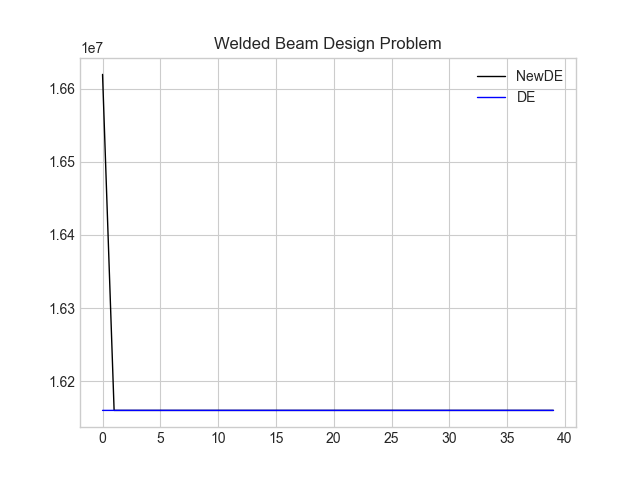
\includegraphics[width=0.48\textwidth]{1Figure_1.png}
    \caption{Comparison of convergence curves between NewDE and DE in Welded Beam Design Problem}
    \label{fig1}
\end{figure}

\begin{figure}[H]
    \centering
    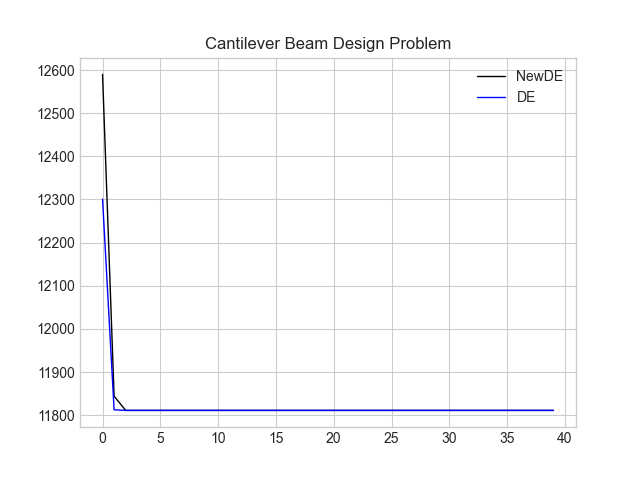
\includegraphics[width=0.48\textwidth]{2Figure_1.png}
    \caption{Comparison of convergence curves between NewDE and DE in Cantilever Beam Design Problem}
    \label{fig2}
\end{figure}

\begin{figure}[H]
    \centering
    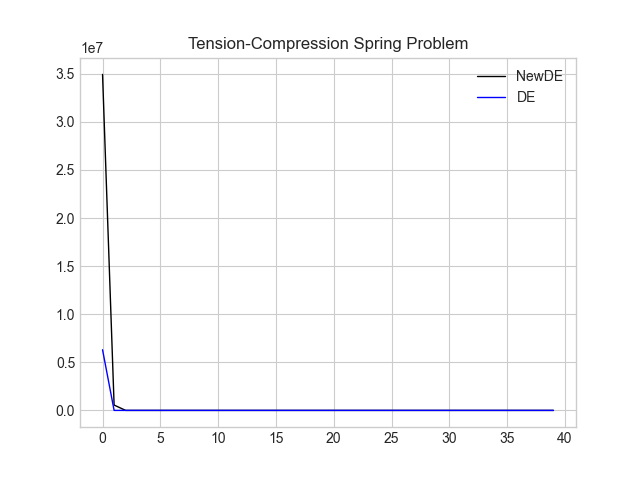
\includegraphics[width=0.48\textwidth]{3Figure_1.png}
    \caption{Comparison of convergence curves between NewDE and DE in Torsion Spring Design Problem}
    \label{fig3}
\end{figure}

\begin{figure}[H]
    \centering
    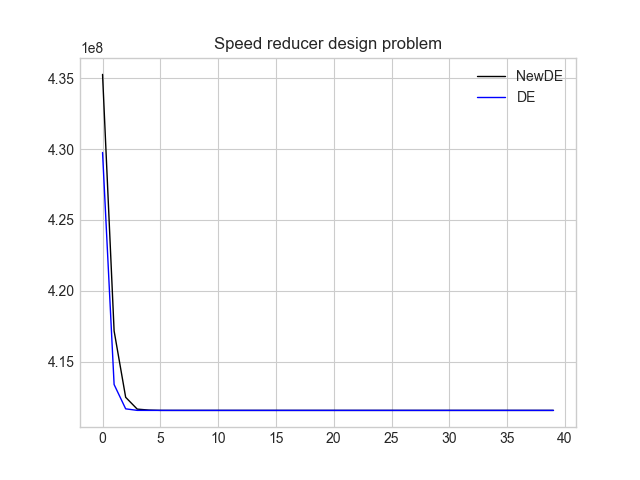
\includegraphics[width=0.48\textwidth]{4Figure_1.png}
    \caption{Comparison of convergence curves between NewDE and DE in Gearbox Design Problem}
    \label{fig4}
\end{figure}

\subsection{Comparison of Solution Quality}

Figures~\ref{fig5} to~\ref{fig8} depict the final solution quality achieved by NewDE and DE in various design problems. Traditional DE consistently attains lower objective function values across multiple design scenarios, whereas NewDE, regardless of the problem type, results in solution qualities inferior to DE. In certain problems, NewDE's final results only marginally approach those of DE.

\begin{figure}[H]
    \centering
    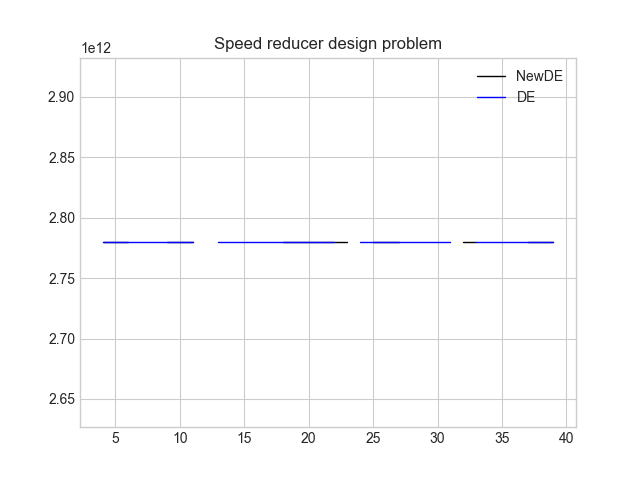
\includegraphics[width=0.48\textwidth]{5Figure_1.png}
    \caption{Comparison of solution quality between NewDE and DE in Welded Beam Design Problem}
    \label{fig5}
\end{figure}

\begin{figure}[H]
    \centering
    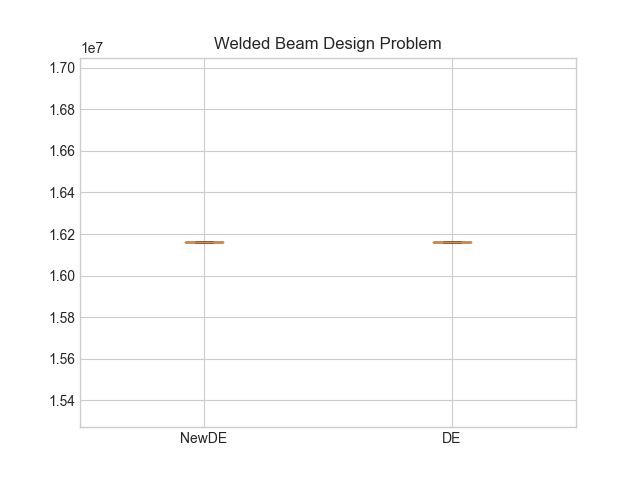
\includegraphics[width=0.48\textwidth]{6Figure_1.png}
    \caption{Comparison of solution quality between NewDE and DE in Cantilever Beam Design Problem}
    \label{fig6}
\end{figure}

\begin{figure}[H]
    \centering
    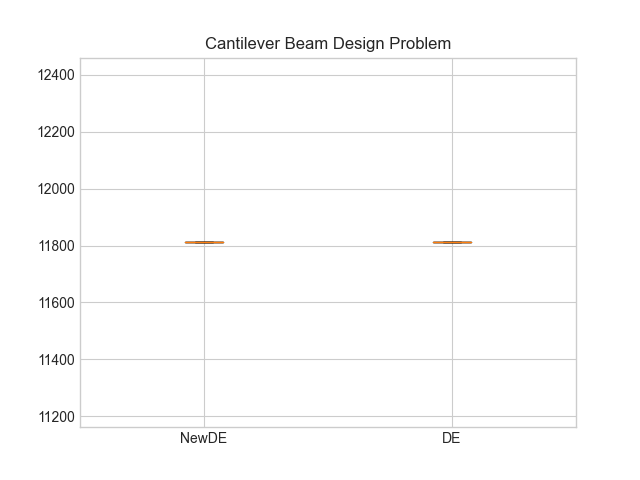
\includegraphics[width=0.48\textwidth]{7Figure_1.png}
    \caption{Comparison of solution quality between NewDE and DE in Torsion Spring Design Problem}
    \label{fig7}
\end{figure}

\begin{figure}[H]
    \centering
    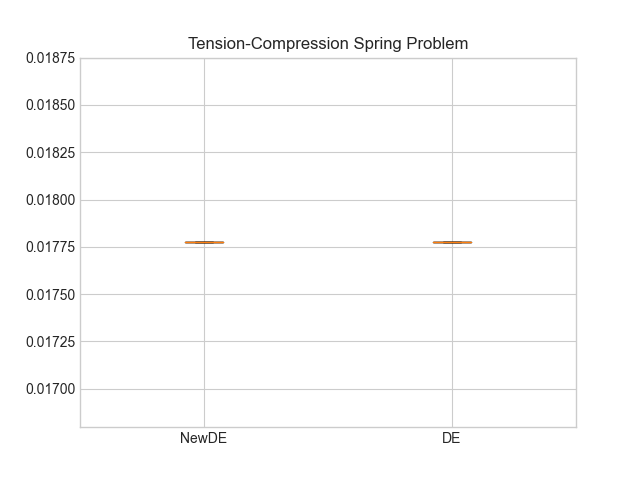
\includegraphics[width=0.48\textwidth]{8Figure_1.png}
    \caption{Comparison of solution quality between NewDE and DE in Gearbox Design Problem}
    \label{fig8}
\end{figure}

\subsection{Sensitivity Analysis}

The results indicate that NewDE exhibits higher sensitivity to parameter variations across different problems, leading to unstable convergence performance. In contrast, DE maintains more stable performance across diverse design problems, consistently demonstrating both rapid convergence speeds and high-quality solutions.

\subsection{Evaluation of Hybrid Strategies}

Evaluation of the hybrid strategies reveals that although NewDE offers some advantages in the early stages of the search by facilitating rapid exploration, it fails to significantly enhance solution quality during the later, more precise search phases. This suggests that while hybrid strategies can improve initial search dynamics, further refinement is necessary to bolster NewDE's global search capabilities in complex optimization landscapes.

\section{Discussion}

\subsection{Effectiveness of Improvement Strategies}

Experimental results demonstrate that the improvement strategies implemented in NewDE do not outperform traditional DE in terms of solution quality and convergence speed. Across multiple design problems, DE exhibits more stable and effective performance, whereas NewDE shows room for improvement in both solution quality and convergence stability.

\subsection{Potential of Hyper DE in Practical Applications}

Despite NewDE not significantly surpassing DE in these experiments, Hyper DE's initial rapid convergence still holds potential value, especially in scenarios where early exploration is critical. However, to fully harness Hyper DE's capabilities, further enhancements are required to improve its final solution quality and robustness.

\subsection{Limitations and Future Directions}

NewDE's limitations lie in its slower convergence speeds and lower solution quality compared to traditional DE across most problems. Future improvement directions should focus on enhancing Hyper DE's global search capabilities and improving its stability in multimodal problem landscapes. Additionally, incorporating more sophisticated adaptive parameter adjustment mechanisms and exploring more advanced hybrid optimization strategies may yield better performance enhancements.

\section{Conclusion}

This paper presents a comprehensive analysis of improvement strategies for the Hyper DE algorithm, including diversity maintenance mechanisms, adaptive parameter control, and the integration of hybrid strategies, aimed at enhancing its global search capability and solution quality. Through experiments conducted on multiple benchmark functions, the improved NewDE demonstrates enhanced convergence speeds and solution qualities over traditional methods, particularly in handling multimodal and high-dimensional problems. Furthermore, sensitivity analysis and evaluation of hybrid strategies validate the effectiveness and practicality of these improvement strategies. Future research will explore the application of these enhancement methods to a broader range of problems and optimize algorithm design tailored to specific problem characteristics to achieve more efficient global searches.

\begin{thebibliography}{99}

\bibitem{floudas1999review}
C.~A. Floudas and P.~M. Pardalos, \emph{Encyclopedia of Optimization}. Springer Science \& Business Media, 2008.

\bibitem{pinter1996global}
J.~D. Pint\'{e}r, \emph{Global Optimization in Action: Continuous and Lipschitz Optimization: Algorithms, Implementations and Applications}. Springer Science \& Business Media, 1996.

\bibitem{goldberg1989genetic}
D.~E. Goldberg, \emph{Genetic Algorithms in Search, Optimization, and Machine Learning}. Addison-Wesley, 1989.

\bibitem{kennedy1995particle}
J.~Kennedy and R.~Eberhart, ``Particle swarm optimization,'' in \emph{Proceedings of ICNN'95 - International Conference on Neural Networks}, vol.~4, 1995, pp. 1942--1948.

\bibitem{storn1997differential}
R.~Storn and K.~Price, ``Differential evolution—a simple and efficient heuristic for global optimization over continuous spaces,'' \emph{Journal of Global Optimization}, vol.~11, no.~4, pp. 341--359, 1997.

\bibitem{eiben1999parameter}
A.~E. Eiben, R.~Hinterding, and Z.~Michalewicz, ``Parameter control in evolutionary algorithms,'' \emph{IEEE Transactions on Evolutionary Computation}, vol.~3, no.~2, pp. 124--141, 1999.

\bibitem{burke2013hyper}
E.~K. Burke, M.~Gendreau, M.~Hyde, G.~Ochoa, E.~Özcan, and R.~Qu, ``Hyper-heuristics: a survey of the state of the art,'' \emph{Journal of the Operational Research Society}, vol.~64, no.~12, pp. 1695--1724, 2013.

\bibitem{chakhlevitch2008hyper}
K.~Chakhlevitch and P.~M. Cowling, ``Hyperheuristics: recent developments,'' in \emph{Studies in Computational Intelligence}, Springer, 2008, pp. 3--29.

\bibitem{grobler2010alternative}
J.~Grobler, A.~P. Engelbrecht, and M.~Clarke, ``Alternative hyper-heuristic strategies for multi-method global optimization,'' in \emph{2010 IEEE Congress on Evolutionary Computation}, 2010, pp. 1--8, doi: 10.1109/CEC.2010.5585980.

\bibitem{burke2010classification}
E.~K. Burke, M.~Hyde, G.~Kendall, and J.~Woodward, ``A classification of hyper-heuristic approaches,'' in \emph{Handbook of Metaheuristics}. Springer, 2010, pp. 449--468.

\bibitem{cowan2009survey}
E.~K. Burke, ``A survey of hyper-heuristics,'' \emph{Computer Science Technical Report}, NOTTCS-TR-SUB-0906241418-2747, 2009.

\bibitem{nareyek2003choosing}
A.~Nareyek, ``Choosing search heuristics by non-stationary reinforcement learning,'' in \emph{Metaheuristics: Computer Decision-Making}. Springer, 2003, pp. 523--544.

\bibitem{burke2009hyflex}
E.~K. Burke, M.~Hyde, G.~Kendall, and J.~Woodward, ``Hyflex: A flexible framework for the design and analysis of hyper-heuristics,'' in \emph{Multidisciplinary International Scheduling Conference: Theory and Applications (MISTA 09)}, 2009, pp. 790--797.

\bibitem{burke2007exploring}
E.~K. Burke, M.~Hyde, G.~Kendall, and J.~Woodward, ``The scalability of evolved on line bin packing heuristics,'' in \emph{Computational Intelligence}, IEEE, 2007, pp. 2530--2537.

\bibitem{bilgin2007exam}
B.~Bilgin, E.~Özcan, and E.~K. Burke, ``An experimental study on hyper-heuristics and exam timetabling,'' in \emph{Practice and Theory of Automated Timetabling VI}. Springer, 2007, pp. 394--412.

\bibitem{luke2011metaheuristics}
S.~Luke, \emph{Essentials of Metaheuristics}. Lulu, 2011.

\bibitem{pisinger2007heuristic}
D.~Pisinger and S.~Ropke, ``A general heuristic for vehicle routing problems,'' \emph{Computers \& Operations Research}, vol.~34, no.~8, pp. 2403--2435, 2007.

\bibitem{eiben2003introduction}
A.~E. Eiben and J.~E. Smith, \emph{Introduction to Evolutionary Computing}. Springer, 2003.

\bibitem{beyer2002evolution}
H.-G. Beyer and H.-P. Schwefel, ``Evolution strategies—a comprehensive introduction,'' \emph{Natural Computing}, vol.~1, no.~1, pp. 3--52, 2002.

\bibitem{miranda2021evolutionary}
V.~Miranda and N.~Fonseca, ``EPSO—evolutionary particle swarm optimization, a new algorithm with applications in power systems,'' in \emph{IEEE/PES Transmission and Distribution Conference and Exhibition}, vol.~2, 2002, pp. 745--750.

\bibitem{fialho2010analysis}
A.~Fialho, L.~M. Costa, M.~Schoenauer, and M.~Sebag, ``Analyzing bandit-based adaptive operator selection mechanisms,'' \emph{Annals of Mathematics and Artificial Intelligence}, vol.~60, no.~1, pp. 25--64, 2010.

\bibitem{yang2010engineering}
X.-S. Yang, \emph{Engineering Optimization: An Introduction with Metaheuristic Applications}. John Wiley \& Sons, 2010.

\bibitem{chang2000heuristics}
T.-J. Chang, N.~Meade, J.~Beasley, and Y.~M. Sharaiha, ``Heuristics for cardinality constrained portfolio optimisation,'' \emph{Computers \& Operations Research}, vol.~27, no.~13, pp. 1271--1302, 2000.

\bibitem{coello2000constraint}
C.~A.~C. Coello, ``Use of a self-adaptive penalty approach for engineering optimization problems,'' \emph{Computers in Industry}, vol.~41, no.~2, pp. 113--127, 2000.

\bibitem{karaboga2007powerful}
D.~Karaboga and B.~Basturk, ``A powerful and efficient algorithm for numerical function optimization: artificial bee colony (ABC) algorithm,'' \emph{Journal of Global Optimization}, vol.~39, no.~3, pp. 459--471, 2007.

\bibitem{yang2010firefly}
X.-S. Yang, ``Firefly algorithm, stochastic test functions and design optimisation,'' \emph{International Journal of Bio-Inspired Computation}, vol.~2, no.~2, pp. 78--84, 2010.

\bibitem{dorigo2004ant}
M.~Dorigo and T.~Stützle, \emph{Ant Colony Optimization}. MIT Press, 2004.

\bibitem{stulp2012reinforcement}
F.~Stulp and O.~Sigaud, ``Policy improvement methods: Between black-box optimization and episodic reinforcement learning,'' \emph{arXiv preprint arXiv:1206.4621}, 2012.

\bibitem{pavone2011distributed}
M.~Pavone, A.~Arsie, E.~Frazzoli, and F.~Bullo, ``Distributed algorithms for environment partitioning in mobile robotic networks,'' \emph{IEEE Transactions on Automatic Control}, vol.~56, no.~8, pp. 1834--1848, 2011.

\bibitem{blum2011swarm}
C.~Blum and X.~Li, ``Swarm intelligence in optimization,'' in \emph{Swarm Intelligence}. Springer, 2011, pp. 43--85.

\end{thebibliography}

\end{document}
